\section{Katalog Wahrscheinlichkeitsverteilungen}

\subsection[Übersicht Zufallsprozesse -- Verteilungen]{Übersicht Zufallsprozesse \textrightarrow\ Verteilungen}

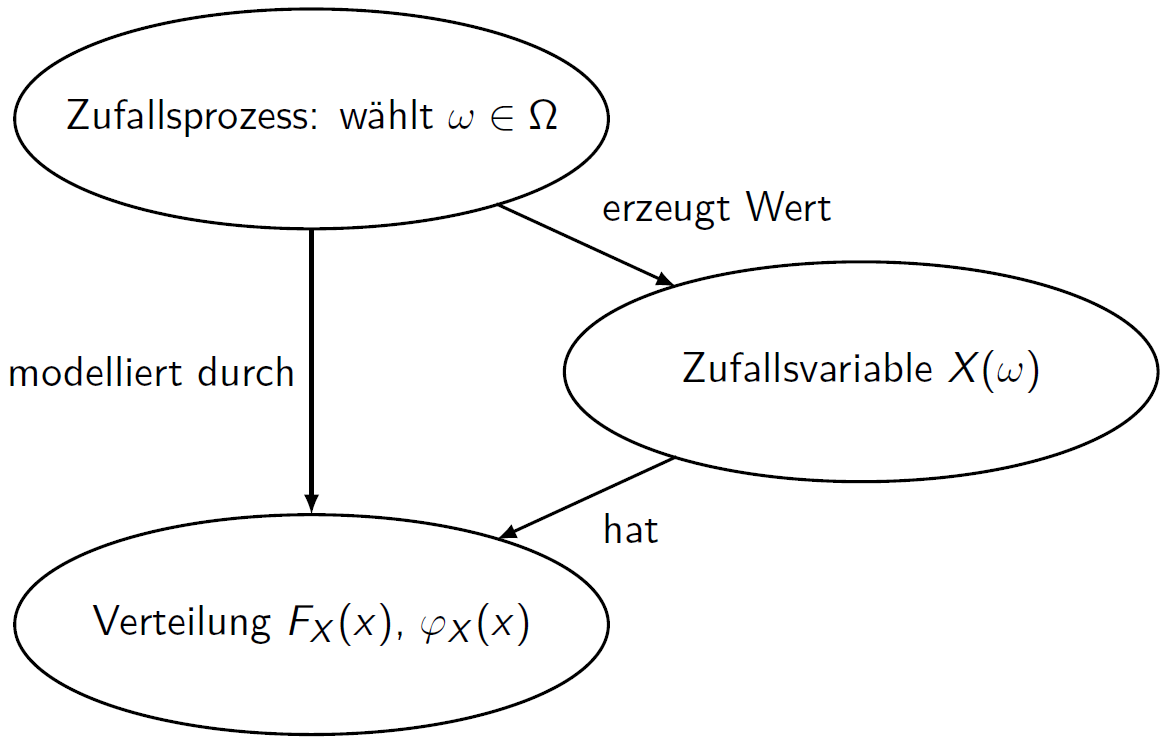
\includegraphics[width=0.5\columnwidth]{images/uebersicht_zufallsprozesse_verteilung}

% Platz für eigene Notizen...


\subsection{Gedächtnislose Prozesse}

\subsubsection{Definition}

Die positive Zufallsvariable $T$ ist der Zeitpukt, zu dem ein Ereignis eintritt

\vspace{0.2cm}

\begin{minipage}{0.38\columnwidth}
	$$ \boxed{ F(x) = P( T \leq x ) } $$
\end{minipage}
\hfill
\begin{minipage}{0.58\columnwidth}
	$$ \boxed{ G(x) = 1 - F(x) = P(T > x) } $$
\end{minipage}


\subsubsection{Gedächtnislos}

$T$ ist gedächtnislos, wenn die Wahrscheinlichkeit, dass das Ereignis in einem Intervall eintritt, immer gleich gross ist, 
wenn es zu Beginn des Intervalls noch nicht eingetreten ist \\
\textbf{Bei gedächtnislosen Prozessen hat die Vergangenheit keinen Einfluss auf den Ausgang eines Experiments / Prozesses }

$$ \cbl{P(T \leq x+y \, | \, T > x)} = \cgn{P(T \leq y)} $$

\cgn{Wahrscheinlichkeit, dass Ereingnis jetzt eintritt} \\
\cbl{Wahrscheinlichkeit, dass Ereingnis später eintritt}

\vspace{0.1cm}

\textrightarrow\ \textbf{Exponentialverteilung} erfüllt diese Bedingung


\subsubsection{Beispiele für Gedächtnislose Prozesse}

\begin{tabular}{lll}
	\tabitem Etwas geht kaputt	& \tabitem Radioaktiver Zerfall	& \tabitem Warteschlangen 
\end{tabular}


\subsection{Exponentialverteilung (gedächtnislos)}

\begin{minipage}[c]{0.46\columnwidth}
	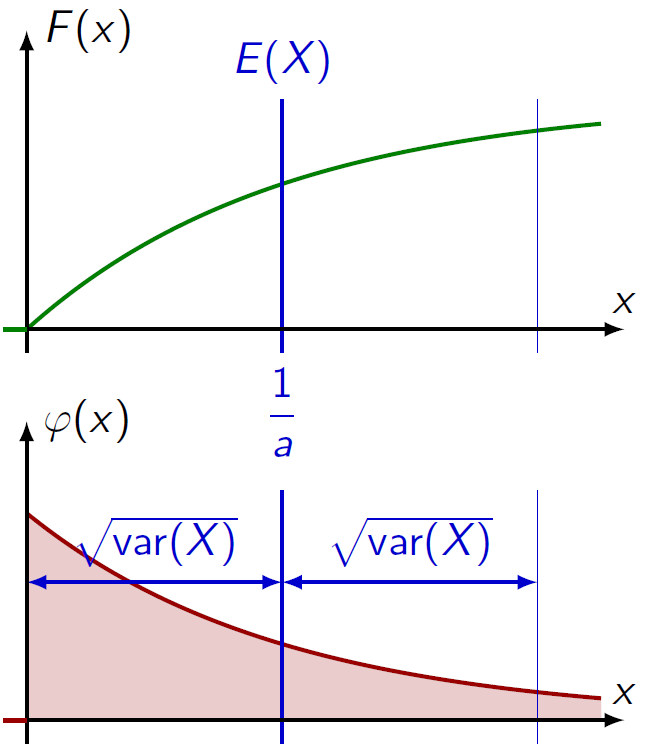
\includegraphics[width=\columnwidth]{images/exponentialverteilung.png}
\end{minipage}
\hfill
	\begin{minipage}[c]{0.52\columnwidth}
	$\cgn{F(x)} = \begin{cases} 
		0 				& x \leq 0 \\
		1 - e^{-a\, x} 	& x > 0 
	\end{cases}$

	\vspace{0.3cm}

	$\crd{\varphi(x)} = \begin{cases} 
		0 					& x \leq 0 \\
		a \, e^{-a \, x} 	& x > 0 
	\end{cases}$ 

	\vspace{0.3cm}

	Parameter: \quad $a$, $\frac{1}{a}$

	\vspace{0.2cm}

	$\frac{1}{a} = $ MTBF (Mean Time Between Failure) \\
	\textbf{( \textrightarrow\ mittlere Lebnsdauer)}
\end{minipage}


\subsubsection{Eigenschaften der Exponentialverteilung}

\myul{\textbf{Erwartungswert $\bm{E(X)}$}}
$$ \boxed{ E(X) = \frac{1}{a} = \text{MTBF (mittlere Lebensdauer)} } $$

\myul{\textbf{Varianz $\bm{\var(x)}$}}

\vspace{0.2cm}

\begin{minipage}[c]{0.6\columnwidth}
	$$ \boxed{ \sigma^2 = \var(x) = E(X^2) - E(X)^2 = \frac{1}{a^2} } $$
\end{minipage}
\hfill
\begin{minipage}[c]{0.36\columnwidth}
	$$ \boxed{E(X^2) = \frac{2}{a^2} } $$
\end{minipage}

\vspace{0.2cm}

\myul{\textbf{Median (Halbwertszeit) }} $\bm{t_{\frac{1}{2}}}$

\begin{minipage}[c]{0.48\columnwidth}
	$$ P(T \leq t_{\frac{1}{2}} ) = \frac{1}{2} $$
\end{minipage}
\hfill
\begin{minipage}[c]{0.48\columnwidth}
	$$ \boxed{ t_{\frac{1}{2}} = \frac{\ln(2)}{a} } $$
\end{minipage}


\subsubsection{Anwendungen}

\begin{tabular}{ll}
	\tabitem Prozess ohne Erinnerungsvermögen	& \tabitem Radioaktivität
\end{tabular}


\subsection{Erlang-Verteilung}

\subsubsection{Voraussetzungen}

$X_i$ ist eine \textbf{unabhängige exponentialverteilte} Zufallsvariable mit Parameter $a$


\subsubsection{Definition der Erlang-Verteilung}

\begin{minipage}[c]{0.48\columnwidth}
	$\crd{\varphi_k(x)} = \begin{cases} 
		0 											& x < 0 \\
		a^k \, \frac{x^{k-1}}{(k-1)!}\, e^{-a \, x} & x \geq 0 
	\end{cases}$ 
\end{minipage}
\hfill
\begin{minipage}[c]{0.48\columnwidth}
	$k = 1$: Exponentialverteilung
\end{minipage}


\subsubsection{Eigenschaften der Erlang-Verteilung}

\myul{\textbf{Verteilungsfunktion $\bm{\varphi_{k+1}(x)}$ von $\bm{T_1 + T_k}$}}
$$ \boxed{ \varphi_{k+1}(x) = \varphi_k * \varphi_1 = a^{k+1} \, \frac{x^k}{k!} \, e^{-a \, x} } $$

\myul{\textbf{Summe von Erwartungswerten $\bm{E(T_1 + T_2)}$}}
$$ \boxed{ E(T_1 + T_2) = E(T_1) + E(T_2) = \frac{1}{a} + \frac{1}{a} = \frac{2}{a} } $$


\subsubsection{Anwendungen}

\begin{tabular}{lll}
	\tabitem Wartezeit in Telefonzentrale / am Postschalter	& \tabitem Warteschlangenprobleme
\end{tabular}


\subsection{Poisson-Verteilung}

\subsubsection{Voraussetzung}

Gedächtnislose Prozesse $T_i$ mit gleichem Parameter $a$


\subsubsection{Aufgabe}

Wie gross ist die Wahrscheinlichkeit, dass in einem Intervall der Länge $x$ genau $k$ Ereignisse / Prozesse stattfinden?
$$ P( S_k \leq x \wedge S_{k+1} > x) = F_k(x) - F_{k+1}(x) \quad \text{mit } S_k = T_1 + ... + T_k $$


\subsubsection{Poisson-Verteilung}

\begin{minipage}{0.36\columnwidth}
	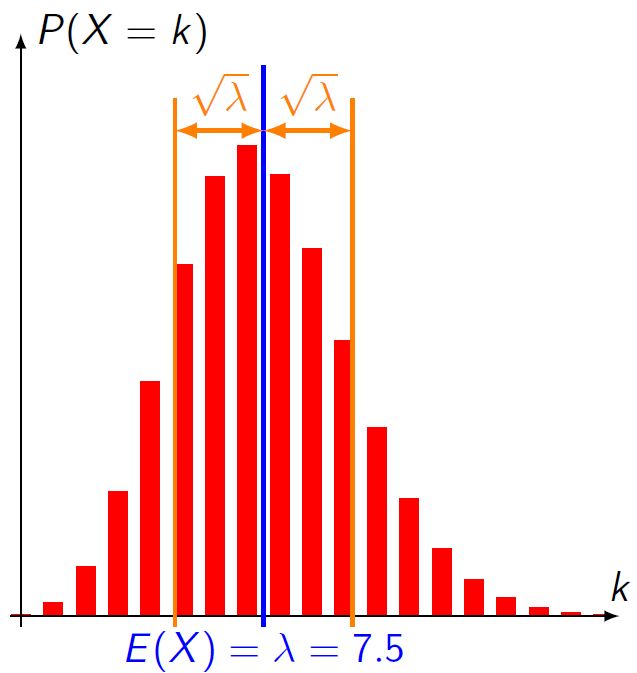
\includegraphics[width=\columnwidth]{images/poissonverteilung.png}
\end{minipage}
\hfill
\begin{minipage}{0.6\columnwidth}
	\begin{align*}
		P_k(\lambda)	&= F_k(x) - F_{k+1}(x)					\\
						&= e^{-a \, x} \frac{(a \, x )^k}{k!} 	\\
		P_k(\lambda) 	&= e^{- \lambda} \frac{\lambda^k}{k!}
	\end{align*}

	Parameter: $\lambda = a \, x$ \\
	(erwartete \# Ereignisse im Intervall $x$)
\end{minipage}


\subsubsection{Eigenschaften der Poisson-Verteilung}

Die Poisson-Verteilung ist eine \textbf{diskrete Verteilung}

\vspace{0.2cm}

\myul{\textbf{Erwartungswert $\bm{E(X)}$}}
\vspace{0.1cm}
$$ \boxed{\lambda = E(X) = a \cdot x } $$

\vspace{0.2cm}

\myul{\textbf{Varianz $\bm{\var(x)}$}}
\vspace{0.1cm}
$$ \boxed{ \sigma^2 = \var(x) = \lambda = a \cdot x } $$

\vspace{0.2cm}

\myul{\textbf{Summe von Wahrscheinlichkeiten (z.B. $\bm{P(k \leq 3)}$) }} 
$$ \boxed{ P(k \leq 3) = e^{-\lambda} \sum\limits_{k=0}^3 \frac{\lambda^k}{k!} } $$


\subsubsection{Anwendungen}

\begin{itemize}
	\item Anzahl Ereignisse mit exponentialverteilten Intervallen
	\item Approximation der Binomialverteilung für seltene Ereignisse, die mit Rate $\lambda$ eintreten
\end{itemize}


\subsection[Zufallszahlen mit Verteilung F(x)]{Zufallszahlen mit Verteilung $F(x)$}

\subsubsection{Voraussetzung}

$F(X)$ ist eine Verteilungsfunktion, $X$ ein im Intervall $[0,1]$ gleichverteilte Zufallsvariable


\subsubsection{Verteilungsfunktion von $Z$}

\begin{minipage}{0.25\columnwidth}
	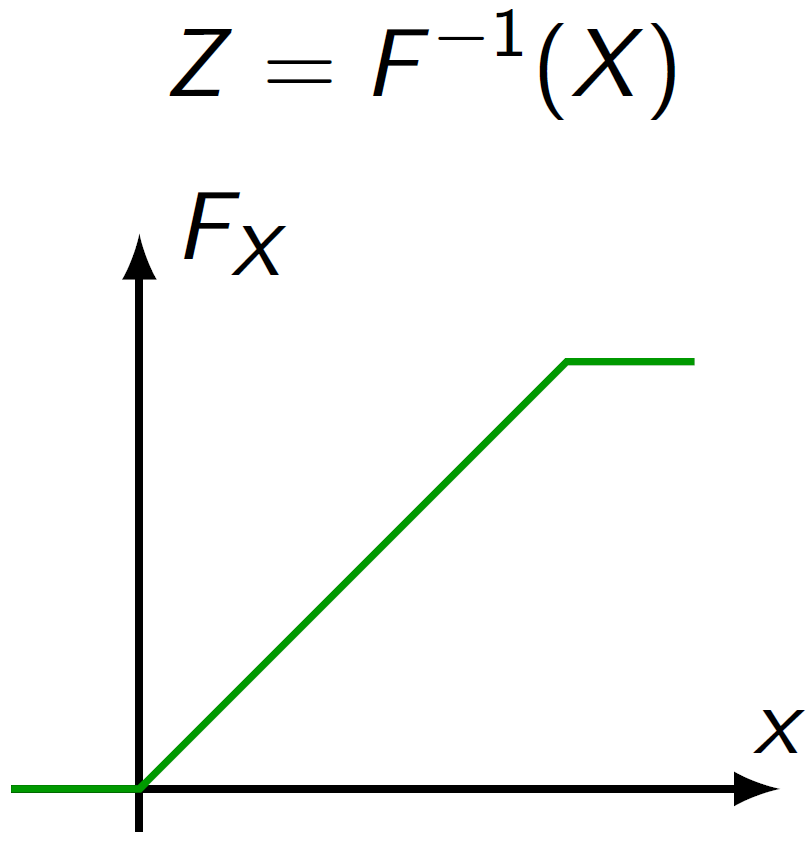
\includegraphics[width=\columnwidth]{images/verteilung_F(x).png}
\end{minipage}
\hfill
\begin{minipage}{0.7\columnwidth}
	\renewcommand{\arraystretch}{1.3}
	\begin{tabular}{r l l}
		$F_Z(z)$ 	& $= P( Z \leq z)$ 			& Definition $F_z$	\\
					& $= P(F^{-1}(X) \leq z)$ 	& Definition $Z$ 	\\
					& $= P(X \leq F(z))$ 		& Umformung 		\\
					& $= F_X(F(z))$ 			& Definition $F_X$ 	\\
					& $= F(z)$   
	\end{tabular}
	\renewcommand{\arraystretch}{1}
\end{minipage}


\subsection{Normalverteilung}

Es geht um eine \textbf{Summe vieler kleiner Einflüsse}

\vspace{0.2cm}

\begin{minipage}{0.4\columnwidth}
	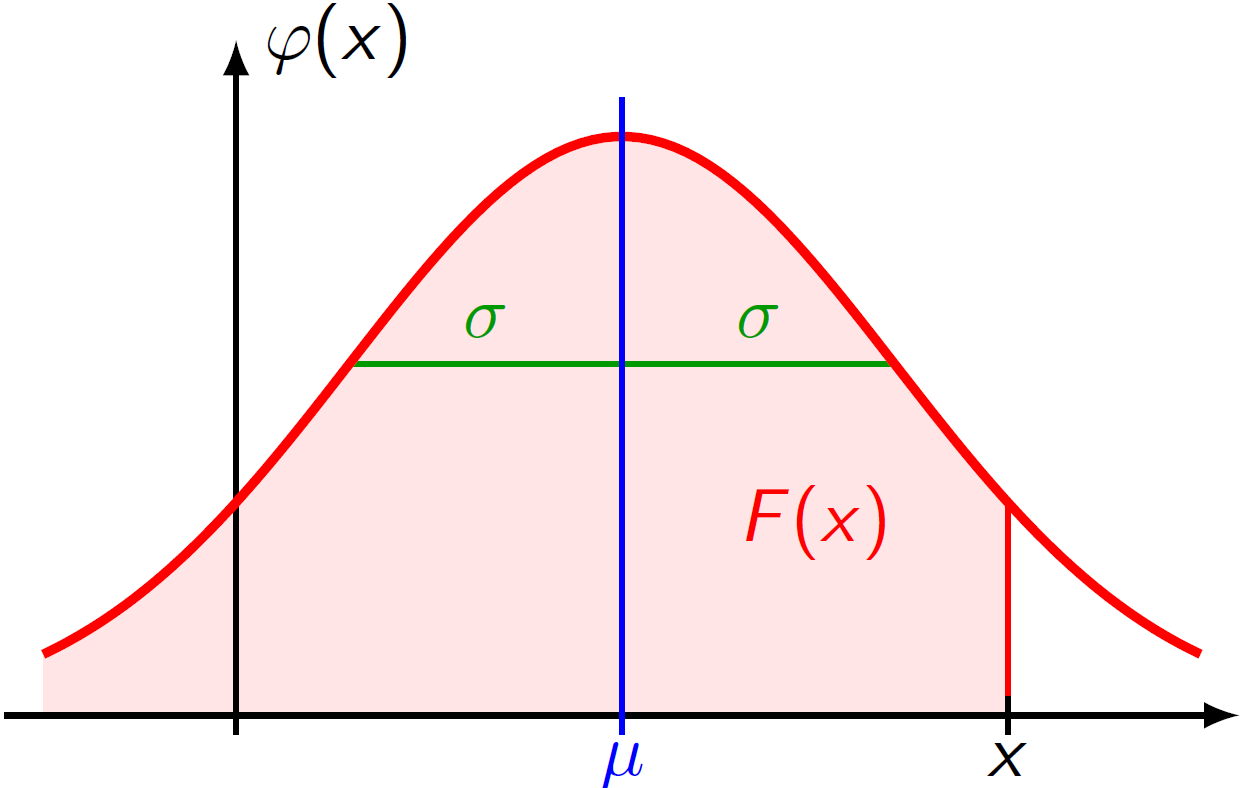
\includegraphics[width=\columnwidth]{images/normalverteilung.png}
	Maximum bei $x = \mu$ \\
	Wendepunkte bei $x = \mu \pm \sigma$ 
\end{minipage}
\hfill
\begin{minipage}{0.48\columnwidth}
	$X$ heisst \textbf{normalverteilt}, mit $E(X) = \mu$ und $\var(X) = \sigma^2$, $N(\mu, \sigma^2)$, wenn sie folgende 
	Wahrscheinlichkeitsdichte $\varphi(x)$ hat:
	$$ \boxed{ \varphi(x) = \frac{1}{\sigma \sqrt{2 \pi}} e^{- \frac{(x - \mu)^2}{2 \sigma^2}} } $$

	$\mu$ \quad Erwartungswert \\
	$\sigma$ \quad Standardabweichung 
\end{minipage}


\subsubsection{Typische Werte der Normalverteilung}

\begin{minipage}{0.45\columnwidth}
	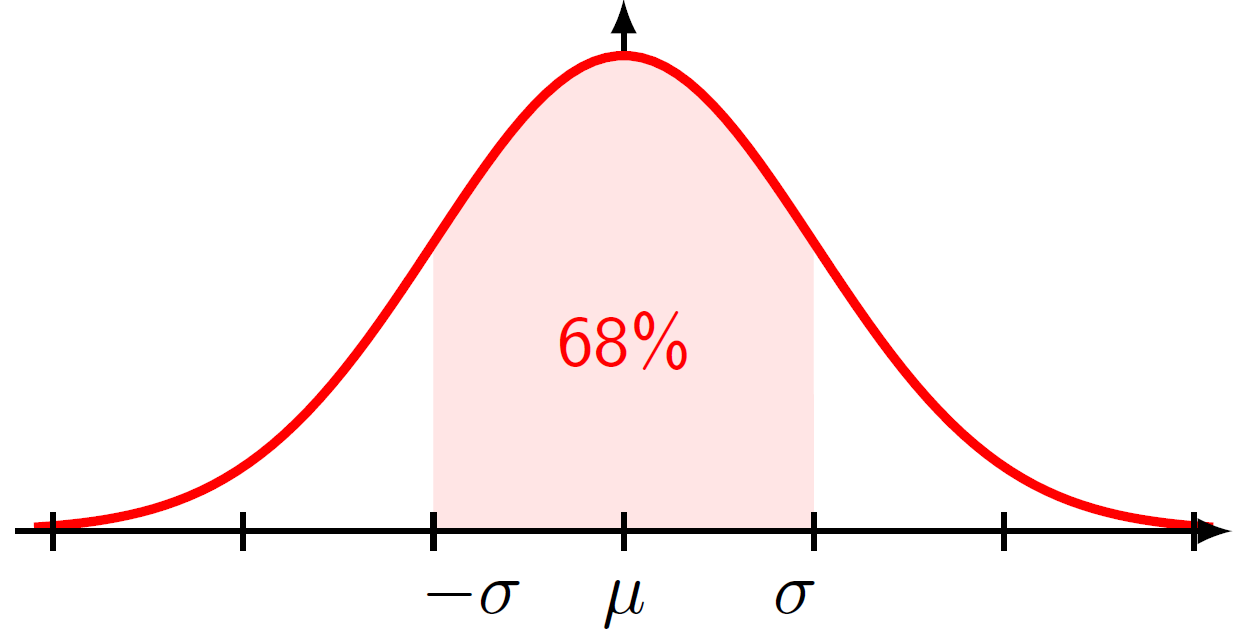
\includegraphics[width=\columnwidth]{images/normalverteilung_typische_werte.png}
\end{minipage}
\hfill
\begin{minipage}{0.45\columnwidth}
	\begin{tabular}{l c l}
		$\pm \, 1 \, \sigma$ & \textrightarrow\ & $68 \, \%$ 	\\
		$\pm \, 2 \, \sigma$ & \textrightarrow\ & $95 \, \%$ 	\\
		$\pm \, 3 \, \sigma$ & \textrightarrow\ & $99.7 \, \%$
	\end{tabular}
\end{minipage}


\subsubsection{Eigenschaften der Normalverteilung}

\myul{\textbf{Wahrscheinlichkeit}}

\vspace{0.1cm}

Wahrscheinlichkeit dafür, dass $X$ zwischen $a$ und $b$ liegt:
$$ P(a < X \leq b) = \frac{1}{\sigma \sqrt{2 \pi}} \int\limits_a^b e^{- \frac{(x - \mu)^2}{2 \sigma^2}}  \, \diff x $$


\myul{\textbf{Keine Stammfunktion}}

\vspace{0.1cm}

Die Wahscheinlichkeitsdichte $\varphi(x)$ der Normalverteilung hat keine Stammfunktion in geschlossener Form\\ 
\textrightarrow\ Nur numerische Berechnungen möglich oder \textbf{Tabellen} verwenden

\vspace{0.2cm}

\myul{\textbf{Symmetrie}}

\vspace{0.1cm}

Die Wahscheinlichkeitsdichte $\varphi(x)$ ist \textbf{symmetrisch} bezüglich $x = \mu$ \\
\textrightarrow\ Erwartungswert $E(X) = \mu$


\subsubsection{Anwendungen}

\begin{itemize}
	\item \textbf{Summe vieler kleiner Einflüsse} vergl. grosse Varianz
	\item Messwerte
	\item Approximation der Binomialverteilung
\end{itemize}


\subsection{Standardnormalverteilung}

\subsubsection{Standardisierung}

$X$ normalverteilt, mit $E(X) = \mu$, $\var(X) = \sigma^2$, dann ist $Z$ normalverteilt:

\vspace{0.2cm}

\begin{minipage}[t]{0.48\columnwidth}
	$$ \boxed{ Z = \frac{X - \mu}{\sigma} } $$
\end{minipage}
\hfill
\begin{minipage}[t]{0.48\columnwidth}
	\myul{\textbf{Eigenschaften}}

	\vspace{0.1cm}

	\begin{itemize}
		\item $E(Z) = 0$
		\item $\var(Z) = 1$
	\end{itemize}
\end{minipage}


\subsubsection{Verteilungsfunktion $\Phi$  der Standardnormalverteilung}

\begin{minipage}{0.48\columnwidth}	
	$$ \boxed{ \Phi(z) = P(Z \leq z) } $$
\end{minipage}
\hfill
\begin{minipage}{0.48\columnwidth}
	$$ \boxed{ \Phi(-z) = 1 -  \Phi(z) } $$
\end{minipage}


\example{Standardnormalverteilung}

\vspace{-0.4cm}

\begin{align*}
	P(\cbl{a} < X \leq \cor{b})	&= P \left( \frac{\cbl{a} - \mu}{\sigma} < \frac{X - \mu}{\sigma} \leq \frac{\cor{b} - \mu}{\sigma}  \right) 	\\
								&= P \left( \frac{\cbl{a} - \mu}{\sigma}  < Z \leq \frac{\cor{b} - \mu}{\sigma} \right) 						\\
								&= \Phi \Bigg( \frac{\cor{b} - \mu}{\sigma} \Bigg) -  \Phi \Bigg( \frac{\cbl{a} - \mu}{\sigma} \Bigg)
\end{align*}

\textrightarrow\ \textbf{Auswertung von $\bm{\Phi()}$ mittels Tabelle in Abschnitt \ref{Verteilungsfunktion der Normalverteilung} } \\
\textrightarrow\ \textbf{Kompakte $\bm{\Phi()}$-Tabelle in Abschnitt \ref{Quantilentabelle der Standardnormalverteilung} } 


\subsubsection{Quantilentabelle der Standardnormalverteilung / TR-Befehle}
\label{Quantilentabelle der Standardnormalverteilung}

\begin{minipage}[c]{0.4\columnwidth}

	\begin{tabular}{|l|r|}
		\hline
		$p$		&	$x$		\\
		\hline
		0.75	&	0.6745	\\
		0.8		&	0.8416	\\
		0.9		&	1.2816	\\
		0.95	&	1.6449	\\
		0.975	&	1.9600	\\
		0.99	&	2.3263	\\
		0.995	&	2.5758	\\
		0.999	&	3.0902	\\
		0.9995	&	3.2905	\\
		\hline
	\end{tabular}
\end{minipage}
\hfill
\begin{minipage}[c]{0.57\columnwidth}
	\myul{\textbf{TI-nspire Befehle (Scratchpad)}}

	\vspace{0.2cm}

	\begin{tabular}{ll}
		$\Phi(x)$ 		& normCdf($\cbl{a}$, $\cor{b}$, $\mu$, $\sigma$)	\\
						& menu-6-5-2										\\
		\\
		$\Phi^{-1}(p)$ 	& invNorm($p$)										\\
						& menu-6-5-3
	\end{tabular}
\end{minipage}


\subsubsection{Rechenregeln Standardnormalverteilung}

\myul{\textbf{Varianz $\bm{\var(X)}$}}
$$ \boxed{ \sigma^2 = \var(X) = E(X^2) - E(X)^2 } $$ 


\myul{\textbf{Summensatz $ \bm{X = X_1 + X_2}$}}

\vspace{0.1cm}
$X_1$ normalverteilt mit $E(X_1) = \mu_1$ und $\var(X_1) = \sigma_1^2$, \\
$X_2$ normalverteilt mit $E(X_2) = \mu_2$ und $\var(X_2) = \sigma_2^2$, \\
dann ist $X = X_1 + X_2$ normalverteilt mit:

\vspace{0.2cm}

\begin{minipage}[c]{0.48\columnwidth}
	$$ \boxed{ E(X) = \mu_1 + \mu_2 } $$
\end{minipage}
\hfill
\begin{minipage}[c]{0.48\columnwidth}
	$$ \boxed{ \sigma^2 = \var(X)  = \sigma_1^2 + \sigma_2^2 } $$
\end{minipage}

\vspace{0.2cm}

\myul{\textbf{Linearität}}

\vspace{0.1cm}

$X$ normalverteilt mit $E(X) = \mu$ und $\var(X) = \sigma^2$, dann ist $a \, X + b$ normalverteilt mit:

\vspace{0.2cm}

\begin{minipage}[c]{0.48\columnwidth}
	$$ \boxed{ E(a \, X + b) = a \, \mu +  b } $$
\end{minipage}
\hfill
\begin{minipage}[c]{0.48\columnwidth}
	$$ \boxed{ \var(a \, X + b)  = a^2 \, \sigma^2 }  $$
\end{minipage}



\subsection[Bestimmung der Parameter]{Bestimmung der Parameter $\bm{\mu}$, $\bm{\sigma^2}$}

\subsubsection{Schätzen}

\vspace{-0.2cm}

$$\hat{\mu} = E(X) = \frac{1}{n} \sum\limits_{i=1}^n x_i \text{  (Mittelwert)}$$
$$\hat{\sigma}^2 = \cor{\frac{n}{n-1}} \, (  E(X^2) - E(X)^2 ) = \cor{\frac{n}{n-1}} \, \left( \frac{1}{n} \sum\limits_{i=1}^n x_i^2 - \Big( \frac{1}{n} \sum\limits_{i=1}^n x_i  \Big)^2  \right) $$

\cor{Korrektur, damit erwartungstreu}


\subsubsection{Wahrscheinlichkeit (Standardnormalverteilung)}

$X \leq x$ mit Wahrscheinlichkeit $p$

\begin{align*}
	P(X \leq x) 														&= p 						\\
	P \Big( \frac{X - \mu}{\sigma} \leq \frac{x - \mu}{\sigma} \Big) 	&= p 						\\
	P \Big( Z \leq \frac{x - \mu}{\sigma} \Big) 						&= p 						\\
	\Phi \Big( \frac{x - \mu}{\sigma} \Big) 							&= p 						\\
	x - \mu 															&= \sigma \, \Phi^{-1}(p) 	\\
	\mu + \Phi^{-1}(p) \, \sigma 										&= x 
\end{align*}

Spezialfall Median: $p = 0.5$ \qquad  $\Phi^{-1}(0.5) = 0$ \qquad \textrightarrow\ $\mu = x$


\subsection{Zentraler Grenzwertsatz (Normalverteilung)}

Sind $X_1$, $X_2, \, \ldots$ identisch verteilte und unabhängige Zufallsvariablen mit $E(X_i) = \mu$ und \\
$\var(X_i) = \sigma^2$, dann gilt:

\renewcommand{\arraystretch}{2}
\begin{tabular}{l c l l}
	$S_n = \sum\limits_{i=1}^n X_i$ 				& \textrightarrow\	& $E(S_n) = n \, \mu$ 	& $\var(S_n) = n \, \sigma^2$	\\
	$Z_n = \frac{S_n - n \, \mu}{\sqrt{n} \sigma}$ 	& \textrightarrow\ 	& $E(Z_n) = 0$ 			& $\var(Z_n) = 1$
\end{tabular}
\renewcommand{\arraystretch}{1}

\vspace{0.2cm}
Für $n \to \infty$ strebt die Verteilung von $Z_n$ gegen die Standardnormalverteilung, d.h. 
$$ \lim\limits_{n \to \infty} P(Z_N \leq z) = \Phi(z) $$
\textbf{\textrightarrow\ Die Summe vieler vergleichbarer kleiner Einflüsse ist annähern normalverteilt}


\subsubsection{Spezielfall Standardnormalverteilung}

$X_i$ Zufallsvariablen mit $E(X_i) = 0$ und $\var(X_i) = 1$, dann konvergiert die Verteilungsfunktion $S_n$
gegen eine Normalverteilung mit $\mu = 0$ und $\sigma = 1$
$$ S_n = \frac{X_1 + \ldots + X_n}{\sqrt{n}} $$
\textbf{\textrightarrow\ Viele kleine Einflüsse ergeben zusammen immer eine Normalverteilung!}

\columnbreak


\subsection{Binomialverteilung}

\subsubsection{Voraussetzungen}

Zufallsexperiment mit \textbf{zwei} möglichen Ausgängen $A$ oder $\overline{A}$ mit \\
Wahrscheinlichkeit $p = P(A)$


\subsubsection{Binomialverteilung}

$X =$ Anzahl Eintreten von $A$ in $n$ \textbf{unabhängigen} Durchführungen

$$ \boxed{ P( X = k ) = \begin{pmatrix} n \\ k \end{pmatrix} p^k (1-p)^{n-k} } $$

\textbf{Notation: } $X \sim \Bi(n, p)$ \\
Taschenrechner Binomialkoeffizient: nCr($n, \, k$) \\
Taschenrechner Binomialverteilung: binomPdf($n, \, p, \,k$)


\subsubsection{Eigenschaften der Binomialverteilung}

\myul{\textbf{Erwartungswert $E(X)$}}

\vspace{0.1cm}

$$ \boxed{ \mu =  E(X) = n \, p } $$

\vspace{0.2cm}

\myul{\textbf{Varianz $\bm{\var(x)}$}}

\vspace{0.1cm}

$$ \boxed{ \sigma^2 = \var(x) = n \, p \, (1 - p) } $$


\subsubsection{Anwendungen}

\begin{itemize}
	\item Anzahl Eintreten eines Bernoulliexperimentes 
\end{itemize}


\subsection{Normalapproximation der Binomialverteilung}

$X$ ist Summe von $n$ kleinen Einflüssen auf das Gesamte \\
\textrightarrow\ $P(X \leq k)$ kann mit der \textbf{Normalverteilung} approximiert werden, sofern die 
\textbf{Anzahl Wiederholungen $\bm{n}$ gross genug} ist und man sich nahe beim 'Buckel' der Normalverteilung befindet

\vspace{0.2cm}

\begin{minipage}[c]{0.48\columnwidth}
	$$ \boxed{ \mu = E(X) = n \, p } $$
\end{minipage}
\hfill
\begin{minipage}[c]{0.48\columnwidth}
	$$ \boxed{ \sigma^2 = \var(X) = n \, p \, (1 - p) } $$
\end{minipage}

\vspace{0.2cm}

$$ \text{ \textrightarrow\ } \frac{X - \mu}{\sigma} = \frac{X - n \, p}{\sqrt{n \, p \, (1 - p)}} \quad \text{ angenähert standardnormalverteilt} $$


\subsubsection{Standardisierung (ohne Korrektur)}

\vspace{-0.4cm}

\begin{align*}
	P(\cbl{a} < X \leq \cor{b}) &= P \left( \frac{\cbl{a} - n \, p}{\sqrt{n p \, (1 - p)}} < \frac{X - n p}{\sqrt{n p (1 - p)}} \leq \frac{\cor{b} - n p}{\sqrt{n p (1 - p)}}  \right) 	\\
								&= P \left( \frac{\cbl{a} - n  p}{\sqrt{n p (1 - p)}}  < Z \leq \frac{\cor{b} - n p}{\sqrt{n p (1 - p)}} \right) 											\\
								&= \Phi \left(  \frac{\cor{b} - n p}{\sqrt{n p (1 - p)}} \right) -  \Phi \left( \frac{\cbl{a} - n p}{\sqrt{n p (1 - p)}} \right)
\end{align*}

\textrightarrow\ \textbf{Auswertung von $\bm{\Phi()}$ mittels Tabelle Abschnitt \ref{Verteilungsfunktion der Normalverteilung}}


\subsubsection{Standardisierung mit Korrektur (Prüfung!)} 

Für eine noch genauerere Approximation kann folgende Korrektur eingefügt werden:

\vspace{-0.2cm}

\begin{align*}
	P(a \, \crd{<} \,  X \,  \cor{\leq} \, b) 	&= \Phi \left( \frac{b \cor{+ \frac{1}{2}} - n \, p}{\sqrt{n p \, (1 - p)}} \right) - \Phi \left( \frac{a \crd{+ \frac{1}{2}} - n p}{\sqrt{n p (1 - p)}} \right) \\
	P(a \, \cgn{\leq} \, X \, \cbl{\leq} \, b) 	&= \Phi \left( \frac{b \cbl{+ \frac{1}{2}} - n \, p}{\sqrt{n p \, (1 - p)}} \right) - \Phi \left( \frac{a \cgn{- \frac{1}{2}} - n p}{\sqrt{n p (1 - p)}} \right)
\end{align*}


\subsubsection{Vergleich \crd{Binomialverteilung} -- \cbl{Normalverteilung}}

\begin{center}
	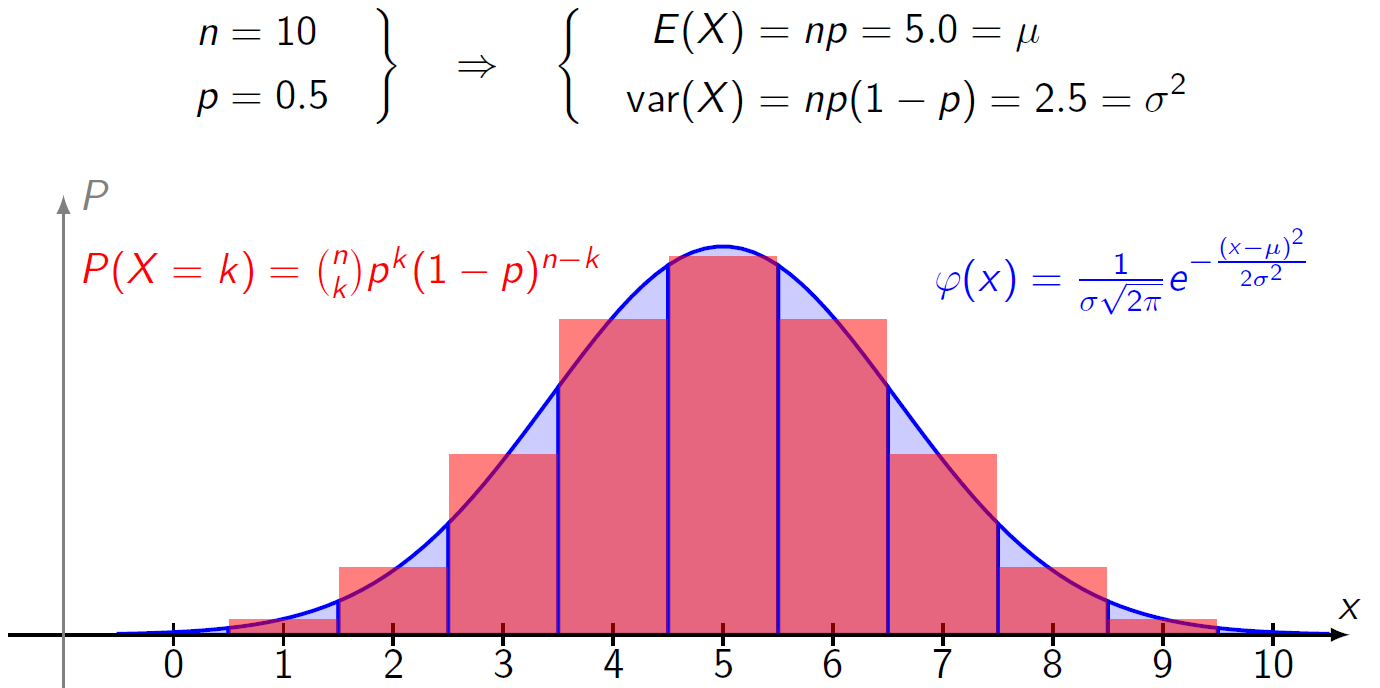
\includegraphics[width=0.75\columnwidth]{images/binomialverteilung_normalverteilung.png}
\end{center}


\columnbreak


\subsection{Approximation für \textbf{seltene} Ereignisse (Poisson)}

\subsubsection{Voraussetzungen}

Grenzwert $n \to \infty$ mit $n \cdot p = \lambda = $ erwartete Anzahl Ereignisse konstant (d.h. $p \to 0$) \\
\textbf{Wenn an der Prüfung \crd{SELTEN} in der Aufgabenstellung steht!!}

$$ \boxed{ P(X = k) = \begin{pmatrix} n \\ k \end{pmatrix} p^k (1-p)^{n-k} = e^{- \lambda} \frac{\lambda^k}{k!} = P_{\lambda}(k) } $$

Parameter: $\lambda = n \cdot p$ \quad (erwartete \# Ereignisse im Intervall $x$)

\vspace{0.2cm}

\myul{\textbf{Poissson - Summe von Wahrscheinlichkeiten (z.B. $\bm{P(k \leq 3)}$) }}
$$ \boxed{ P(k \leq 3) = e^{-\lambda} \sum\limits_{k=0}^3 \frac{\lambda^k}{k!} } $$


\subsection{Hypergeometrische Verteilung}

\subsubsection{Voraussetung}

Von $N$ Objekten sind $M$ markiert. Daraus werden $n$ Objekte zufällig ausgewählt.


\subsubsection{Hypergeometrische Verteilung}

$X = $ Anzahl markierte Objekte unter den zufällig ausgewählten $n$ Objekten \\
Die Wahrscheinlichkeit, dass \textbf{genau $\boldsymbol{m}$ markierte Objekte gezogen} werden lautet:
$$ \boxed{ P(X = m) = \frac{ \begin{pmatrix} M \\ m \end{pmatrix} \begin{pmatrix} N-M \\ n-m \end{pmatrix} }{\begin{pmatrix} N \\ n \end{pmatrix}} } $$
\textbf{Notation: } $X \sim \mathrm{H}(N, M, n) $


\subsubsection{Eigenschaften der Hypergeometrischen Verteilung}

\myul{\textbf{Erwartungswert $\bm{E(X)}$}}

\vspace{0.1cm}

$$ \boxed{ \mu =  E(X) = n \, \frac{M}{N} } $$ 

\vspace{0.2cm}

\myul{\textbf{Varianz $\bm{\var(x)}$}}

\vspace{0.1cm}

$$ \boxed{\sigma^2 =  \var(X) = n \, \frac{M}{N} \Big( 1 - \frac{M}{N} \Big) \frac{N-n}{N-1} } $$


\example{Hypergeometrische Verteilung}

In einer Kiste mit 20 Äpfeln sind 5 wurmstichig. \\
Wie gross ist die Wahrscheinlichkeit, in einer Stichprobe von 8 Äpfel 2 wurmstichtige zu finden? \\
$N = 20$, $M = 5$, $n = 8$, $m = 2$

$$ P(X = 2) = \frac{ \begin{pmatrix} 5 \\ 2 \end{pmatrix} \begin{pmatrix} 15 \\ 6 \end{pmatrix} }{\begin{pmatrix} 20 \\ 8 \end{pmatrix}} = 0.3973 $$


\subsubsection{Begründung Hypergeometrische Verteilung}

\begin{minipage}{0.4\columnwidth}
	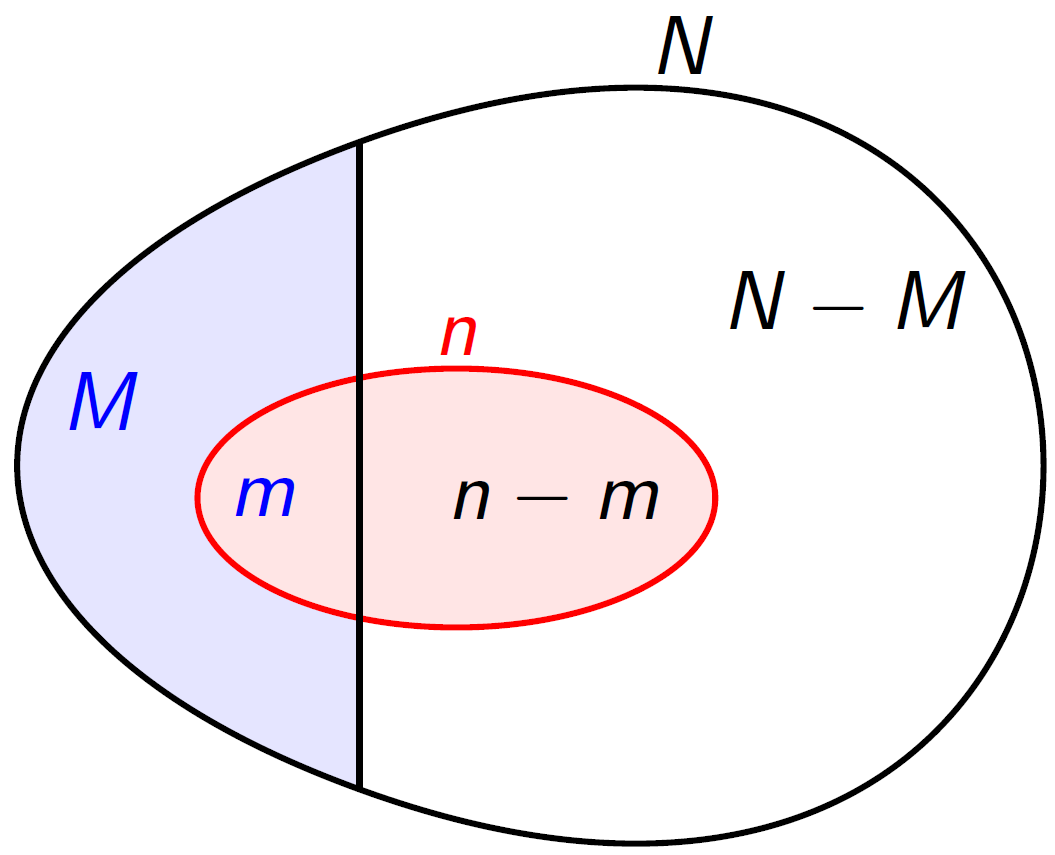
\includegraphics[width=\columnwidth]{images/begruendung_hypergeometrische_verteilung_1.png}
\end{minipage}
\hfill
\begin{minipage}{0.4\columnwidth}
	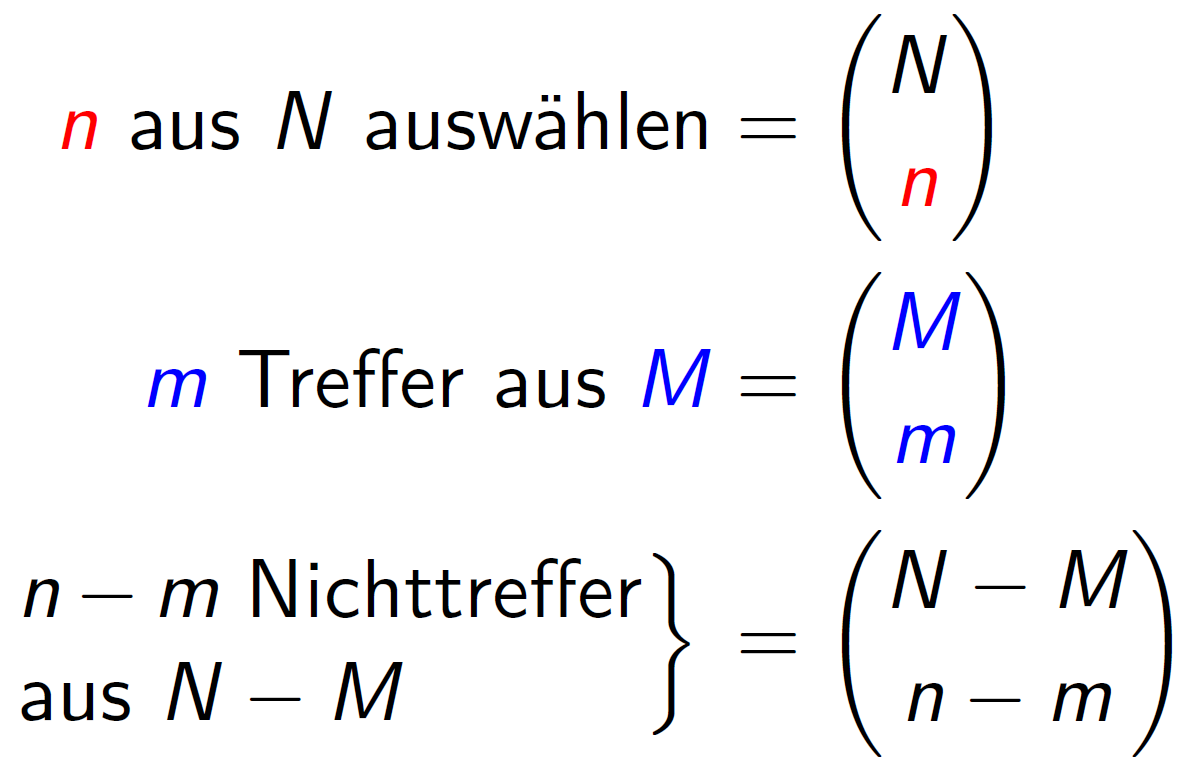
\includegraphics[width=\columnwidth]{images/begruendung_hypergeometrische_verteilung_2.png}
\end{minipage}


\subsection{Potenzverteilung (Skaleninvarianze Prozesse)}

\subsubsection{Skaleninvarianz}

Ein Prozess ist \textbf{skaleninvariant}, wenn er auf jeder Skala \textbf{gleich} abläuft.

\vspace{0.2cm}

Skaliere $x$ mit $b$ \textrightarrow\ Form von $\varphi(x)$ ändert sich nicht

$$ \varphi(bx) = g(b) \, \varphi(x) \quad \text{für } x > x_{\rm min} $$
Faktor $g(b):$ Renormierung


\subsubsection{Potenzverteilung}

\vspace{-0.2cm}

$$ \boxed{ \varphi(x) = C \, e^{- \alpha} \quad \text{mit } \alpha = -g'(1) }$$
Beschränke auf $x > x_{\rm min}$ und wähle $C$ für korrekte Normierung

\vspace{0.2cm}

\begin{minipage}{0.55\columnwidth}
	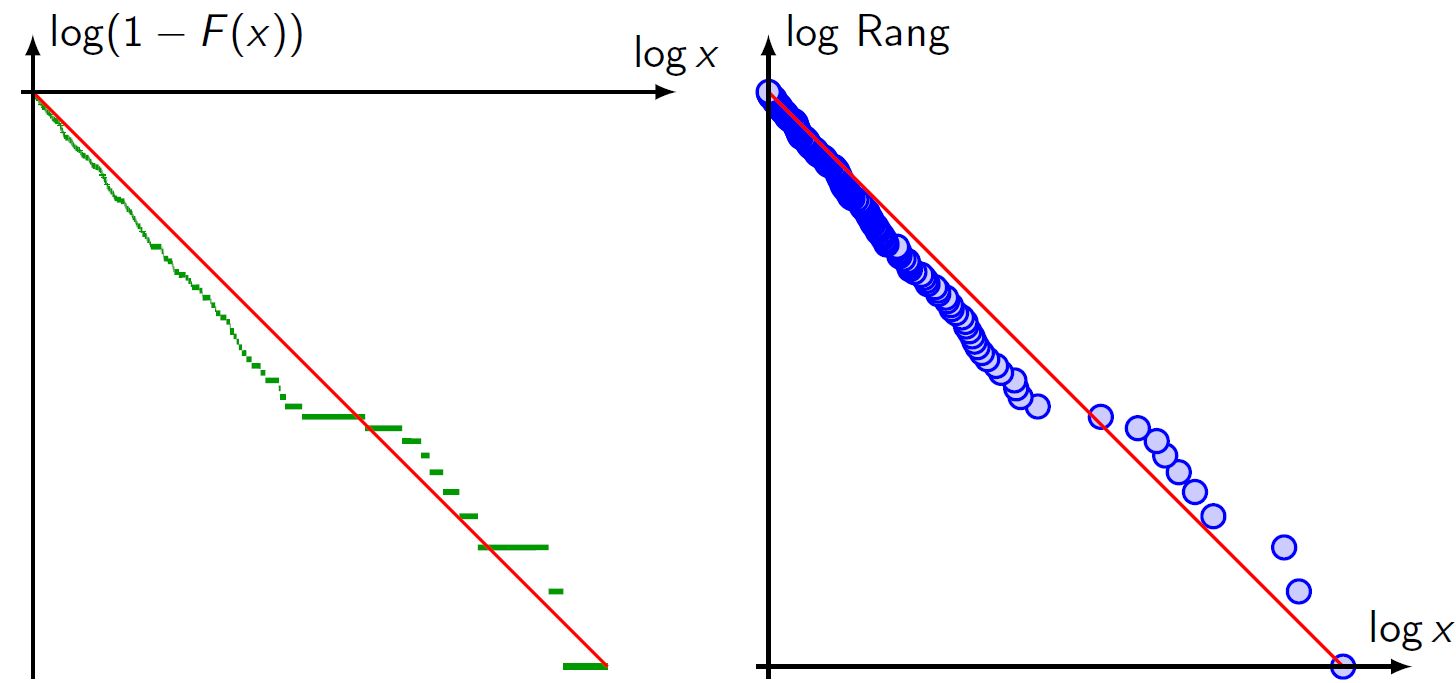
\includegraphics[width=\columnwidth]{images/potenzverteilung.png}
\end{minipage}
\hfill
\begin{minipage}{0.38\columnwidth}
	Geradengleichung in \\
	log-log-Skala
	$$ \log(\varphi(x)) = g'(1) \cdot \log(x) + c $$
\end{minipage}


\subsubsection{Anwendungen}

\begin{minipage}[t]{0.48\columnwidth}
	\begin{itemize}
		\item Städte und Bewohner
		\item Tierarten und ihre Häufigkeit
		\item Mondkrater und Durchmesser
		\item Bücher und Bestseller
	\end{itemize}
\end{minipage}
\hfill
\begin{minipage}[t]{0.48\columnwidth}
	\begin{itemize}
		\item Namen und Häufigkeit
		\item Einkommensverteilung
		\item Skaleninvariante Prozesse
	\end{itemize}
\end{minipage}


\subsubsection{Potenzgesetze für skaleninvariante Prozesse}

\myul{\textbf{Wahrscheinlichkeitsdichte $\bm{\varphi(x)}$}}
$$ \varphi(x) = \begin{cases}
0 																			& x < x_{\rm min} 	\\
\frac{\alpha - 1}{x_{\rm min}} \Big( \frac{x}{x_{\rm min}} \Big)^{-\alpha} 	& x \geq x_{\rm min} 
\end{cases}$$ 


\myul{\textbf{Verteilungsfunktion $\bm{F(x)}$}}

$$ F(x) =  \begin{cases}
0 													& x < x_{\rm min} 		\\
1 - \Big( \frac{x}{x_{\rm min}} \Big)^{1 - \alpha} 	& x \geq x_{\rm min} 
\end{cases}$$ 

\vspace{0.2cm}

\renewcommand{\arraystretch}{1.4}
\begin{tabular}{lll}
	Median 			& $ \mathrm{med}(x) = 2^{\frac{1}{\alpha-1}} \, x_{\rm min} $ 	& für $\alpha > 1$ \\
	Erwartungswert 	& $E(X) = \frac{\alpha - 1}{\alpha - 2} \, x_{\rm min}$ 		& für $\alpha > 2$ \\
	Varianz 		& $ \var(X) = \Big( \frac{\alpha - 1}{\alpha - 3} - \Big( \frac{\alpha - 1}{\alpha - 2} \Big)^2 \Big) \, x_{\rm min}^2 $ & für $\alpha > 3$
\end{tabular}
\renewcommand{\arraystretch}{1}


\subsubsection{'80 / 20 Regel'}

\vspace{-0.4cm}

\begin{minipage}[t]{0.48\columnwidth}
	\begin{align*}
		P(x) 	&= \text{Anteil der Werte } \crd{>} \, x 			\\
				&= 1 - P(X \leq x) = 1 - F(x) 						\\
				&= \int\limits_x^{\infty} \varphi(\xi) \, \diff \xi 
	\end{align*}
\end{minipage}
\hfill
\begin{minipage}[t]{0.48\columnwidth}
	\begin{align*}
		W(x) 	&= \text{Anteil am kumulierten Wert} 									\\
				&= \frac{\int\limits_x^{\infty} \xi \, \varphi(\xi) \, \diff \xi}{E(X)} 
	\end{align*}
	$$ W(x)= P(x)^{\frac{\alpha-2}{\alpha-1}} = P(x)^{\lambda} $$ 
\end{minipage}

\vspace{0.2cm}

\begin{minipage}{0.48\columnwidth}
	$$ \boxed{ \alpha = \frac{\lambda - 2}{\lambda - 1} } $$
\end{minipage}
\hfill
\begin{minipage}{0.48\columnwidth}
	$$ \boxed{ \lambda = \frac{\log(W)}{\log(P)} } $$
\end{minipage}


\subsection{Gleichverteiung}

\begin{minipage}{0.48\columnwidth}
	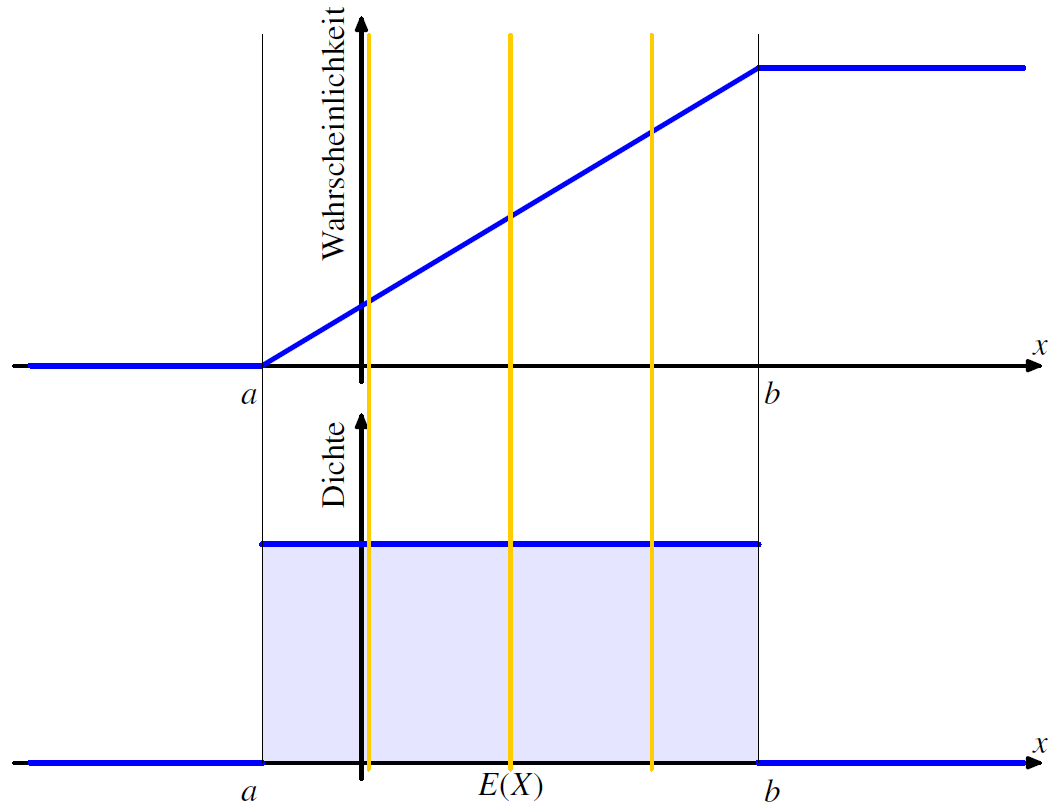
\includegraphics[width=\columnwidth]{images/gleichverteilung.png}
\end{minipage}
\hfill
\begin{minipage}{0.48\columnwidth}
	$\cgn{F(x)} =
	\begin{cases} 
	0 				& x \leq a 			\\
	\frac{x-a}{b-a} & a \leq x \leq b 	\\
	1 				& x > b 
	\end{cases}$ 
	
	\vspace{0.3cm}
	
	$\crd{\varphi(x)} = 
	\begin{cases} 
	\frac{1}{b-a} 	& a \leq x \leq b \\
	0 				& \text{sonst}
	\end{cases}$
\end{minipage}


\subsubsection{Eigenschaften der Gleichverteiung}

\myul{\textbf{Erwartungswert $\bm{E(X)}$}}

$$ \boxed{ E(X) = \frac{a + b}{2}} $$

\vspace{0.2cm}

\textbf{Varianz $\bm{\var(X)}$}

$$ \boxed{\var(X) = \frac{(b - a)^2}{12}} $$


\subsubsection{Anwendungen}

\begin{tabular}{ll}
	\tabitem Verteiung von Zufallszahlen	& \tabitem Keine bevorzugten Werte
\end{tabular}

\columnbreak

